\section{Circuito simple con haz de 3 Conductores}

\begin{figure}[h!]
    \centering
    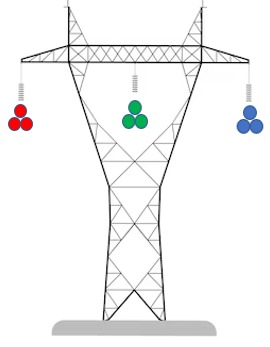
\includegraphics[width=0.48\linewidth]{img/sencillotriplex.jpg}
    \caption{Circuito sencillo 3 conductores disposición horizontal}
    \label{fig:enter-label}
\end{figure}

\begin{figure}[h!]
    \centering
    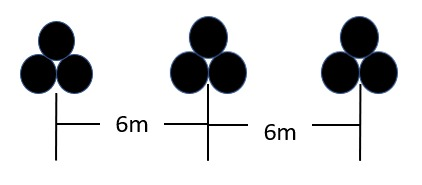
\includegraphics[width=0.48\linewidth]{img/disposicion.jpg}
    \caption{}
    \label{fig:enter-label2}
\end{figure}
\textbf{Datos:}

\begin{align*}
L &= 31~\text{km} & r &= 12,58~\text{mm} \\
S &= 0.4537~[\text{m}] & \alpha_0 &= 0.00438~[\text{mm}] \\
f &= 60~[\text{Hz}] & \text{RMG tabla} &= 9.66~[\text{mm}] \\
R_{\text{AC}75^\circ C} &= 0.106\Omega/\text{km} & V_L &= 230~\text{kV} \\
T_2 &= 28^\circ C & T_1 &= 75^\circ C \\
S &= 700~\text{MVA} & \text{FP} &= 0.9~\text{atraso}
\end{align*}

\begin{align*}
R_{\text{AC}~28^\circ C} &= \left( \frac{1 + \alpha_0 T_2}{1 + \alpha_0 T_1} \right) \cdot R_{\text{75}^\circ C} \\
&= \left( \frac{1 + (0.00438)(28)}{1 + (0.00438)(75)} \right) \cdot 0.106 \\
&= 0.08957~\Omega/\text{km}
\end{align*}

\textbf{Resistencia total por fase:}
\begin{align*}
R_{\text{Fase}} &= \frac{R_{\text{AC}~28^\circ C}}{\text{\#Conductores} \cdot \text{\#Circuitos}} \\
&= \frac{0.08957}{3(1)} = 0.9256~\Omega
\end{align*}

\textbf{Cálculo de la distancia media geométrica:}
\begin{align*}
DMG_{eq} &= \sqrt[3]{D_{12} D_{13} D_{23}} = 7.5595~\text{m}
\end{align*}

\textbf{Radio medio geométrico equivalente de la inductancia:}
\begin{align*}
RMGL_{eq} &= \sqrt[3]{\text{RMG tabla} \cdot S^2} = 0.12639~\text{m}
\end{align*}

\textbf{Inductancia total:}
\begin{align*}
L &= \left(2 \cdot 10^{-4} \right) \ln \left( \frac{DMG_{eq}}{RMGL_{eq}} \right) \\
L &= 8.1823 \cdot 10^{-4}~[\text{H/km/fase}] \\
L_T &= (8.1823 \cdot 10^{-4})(31) = 0.0253~[\text{H/fase}]
\end{align*}

\textbf{Reactancia inductiva:}
\begin{align*}
X_L &= 2\pi \cdot f \cdot L = 2\pi \cdot 60 \cdot 0.0253 = 9.5264~[\Omega] \\
\end{align*}

\textbf{Cálculo de la capacitancia:}

\begin{align*}
C &= \left[ 18 \times 10^9 \cdot \ln \left( \frac{DMG_{eq}}{RMG_{eq}} \right) \right]^{-1} \cdot 1000 \quad [\text{f/km/fase}]
\end{align*}

\textbf{Radio medio geométrico equivalente para la capacitancia:}

\begin{align*}
RMGC_{eq} &= \sqrt[3]{r \cdot s^2} = \sqrt[3]{(12.58 \times 10^{-3})(0.4537)^2} = 0.138
\end{align*}

\begin{align*}
C &= \left[ 18 \times 10^9 \cdot \ln\left( \frac{7.5595}{0.138} \right) \right]^{-1} \cdot 1000 \\begin{align*}
&= 1.3878 \times 10^{-8} \quad [\text{f/km/fase}] \\
\end{align*}

\begin{align*}
C &= (31)(1.3878 \times 10^{-8}) = 4.3022 \times 10^{-7} \quad [\text{f/fase}]
\end{align*}

\begin{align*}
Z_T &= 0.9256 + 9.5624j \quad [\Omega]
\end{align*}

\begin{align*}
Y_T &= 2 \pi f C = 2 \pi \cdot 60 \cdot 4.3022 \times 10^{-7} \cdot j \\
Y_T &= = 1.621 \times 10^{-4} j \quad [\Omega^{-1}]
\end{align*}

\textbf{Constantes de la línea:}

\begin{align*}
A &= 1 + \frac{Z_T Y_T}{2} = 0.9992 \angle 4.30^\circ \\
B &= Z_T \\
C &= Y_T \left( 1 + \frac{Z_T Y_T}{4} \right) = -6.087 \times 10^{-9} + 1.62 \times 10^{-4} j \\
D &= A
\end{align*}


\textbf{Cálculo de corrientes y tensiones:}

\begin{align*}
V_R &= \frac{230}{\sqrt{3}} = 132.79 \angle 0^\circ ~[\text{kV}] \\
I_R &= \left( \frac{700 \cdot 10^6 \angle \cos^{-1}(0.9)^\circ  }{230 \cdot 10^3 \cdot \sqrt{3}} \right) 
= 1757.15 \angle -25.84^\circ~[\text{A}] \\
\\
V_g &= A V_R + B I_R = 142208.219 \angle 5.821^\circ~[\text{V}] \\
I_g &= C V_R + D I_R = 1580.268 - 743.68j~[\text{A}]
\end{align*}

\vspace{1em}

\textbf{Regulación de voltaje:}

\begin{align*}
\%RV &= \left( \frac{ |V_G| }{ |A| \cdot |V_R| } \right) - 1 = 7.17\%
\end{align*}

\vspace{1em}

\textbf{Pérdida de potencia:}

\begin{align*}
PP &= 1.335\%
\end{align*}

\textbf{Efecto corona}
\begin{align*}
U_c &= 4.51 \\
U_{me} &= 264.5 \\
U_c &< U_{me} \quad \Rightarrow \quad \text{Por lo tanto se produce efecto corona}
\end{align*}